\section{Распределенные вычислительные системы}
Парадигма распределенных вычислительных систем в настоящее время характеризуется стремительными темпами развития и эволюции используемых в ней идеологий и подходов. За непродолжительное время существования систем такого типа появилось множество различных схем организаций распределенных вычислений, набравших большой вес и общее признание, но практически исчезнувших впоследствии под давлением более новых и модных подходов. Такая ситуация зачастую ведет к тому, что исчезнувшая из виду технология появляется вновь под новым именем. В результате происходит непрерывное перемешивание базовых концепций с новейшими подходами к разработке. Для изучения и систематизации имеющихся технологий и подходов необходимо разобраться с базовыми понятиями и принципами организации систем подобного направления. 

\subsection{Понятие распределенной системы}
По утверждению известного специалиста в области информатики Э. Таненбаума, не существует общепринятого и в то же время строгого определения распределенной системы. 

Зачастую, при определении понятия <<распределенная система>> главное место отводят принципу разделения функционала между несколькими компьютерами. Однако при таком подходе распределенной является любая вычислительная система, в которой обработка данных разделена между двумя и более компьютерами. Сам Э.~Таненбаум в узком смысле определяет распределенную систему как набор соединенных каналами связи независимых компьютеров, которые с точки зрения пользователя некоторого программного обеспечения выглядяткак единое целое.

\begin{figure}[h]
\center{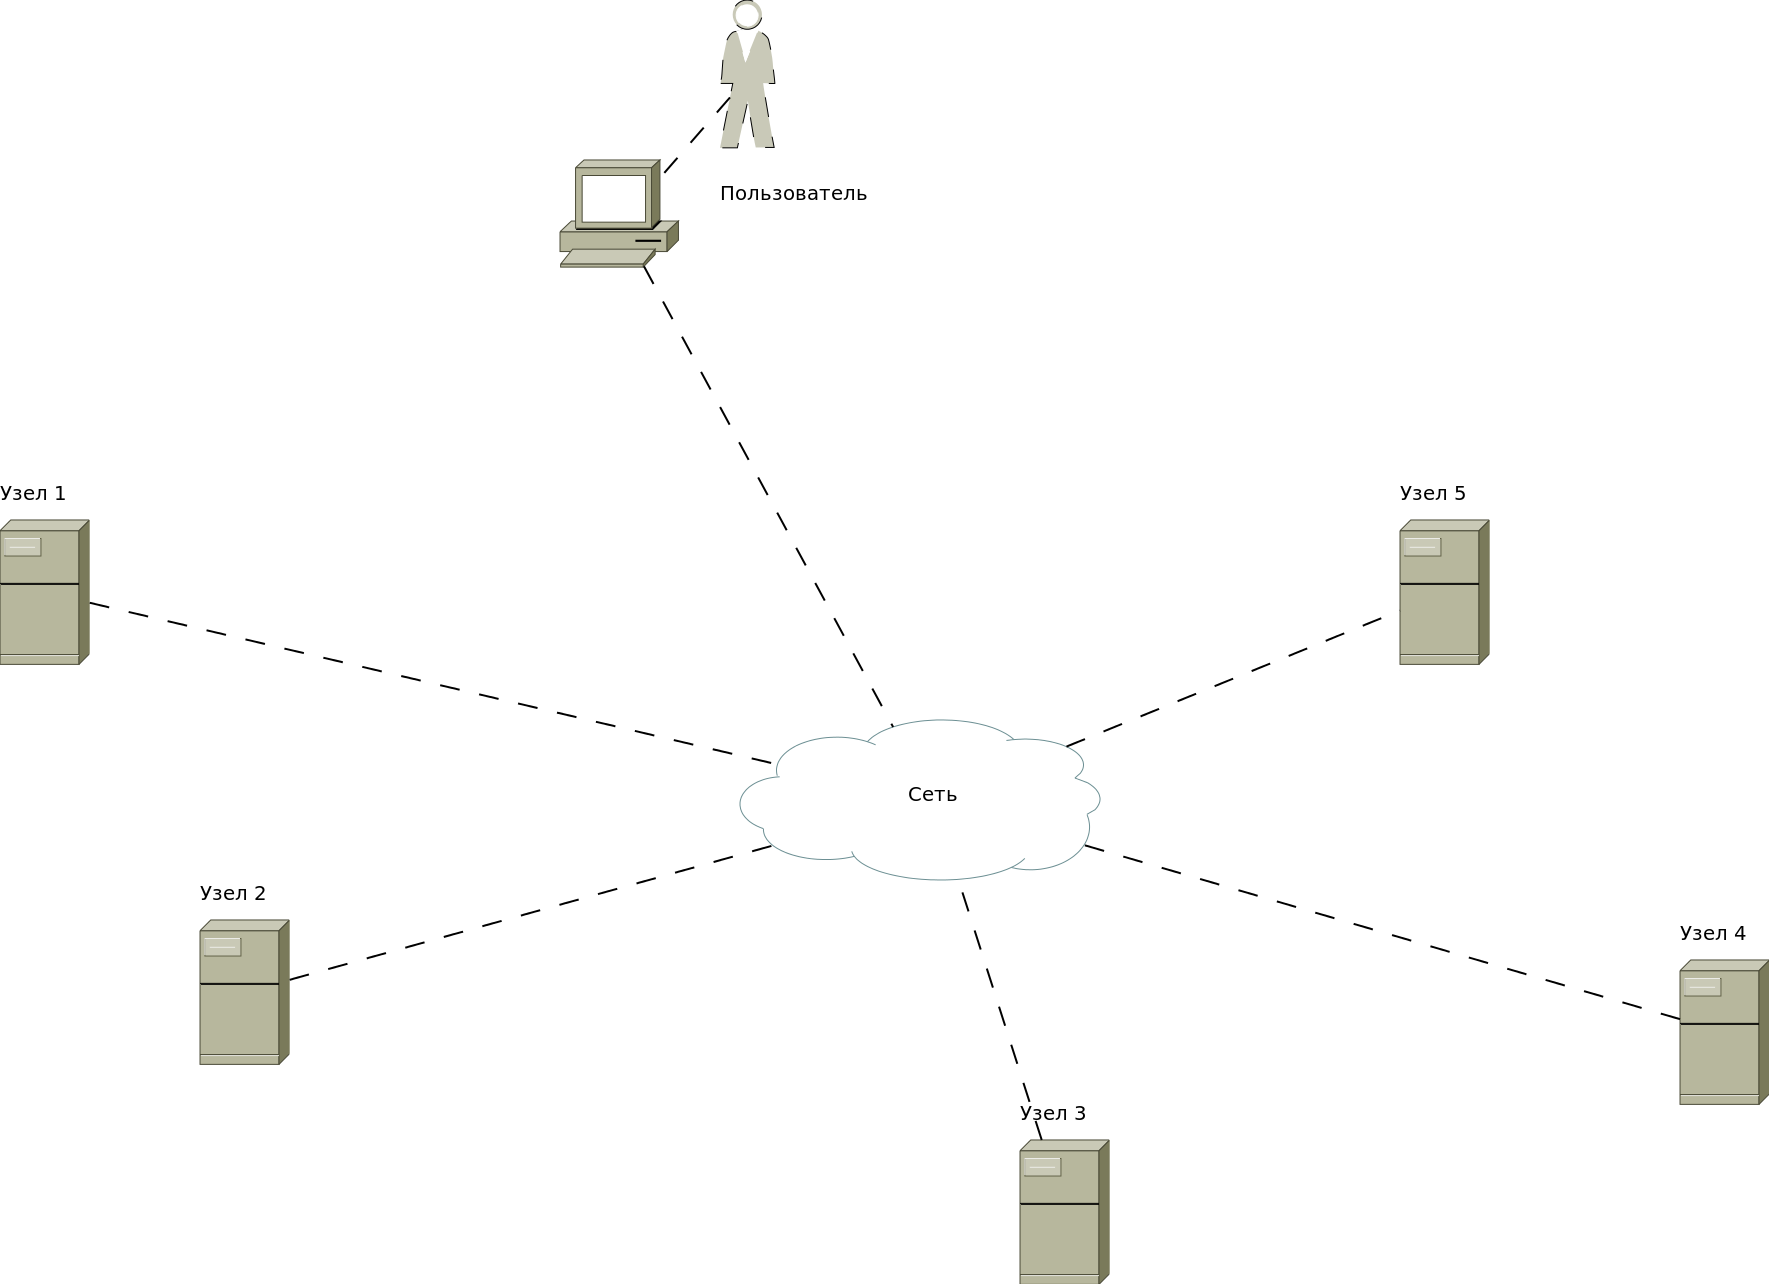
\includegraphics[width=1\linewidth]{dcs}}
\caption{Архитектура распределенной системы}
\label{0:dcs}
\end{figure}

В распределенных системах ключевым моментом является скрытие от пользователей различий между компьютерами и принципов организации их соединений (пользователь может даже не знать, что компьютер, используемый в системе, всего один). Пользователи и приложения единообразно работают в распределенных системах, независимо от того, где и когда происходит их взаимодействие. Вычислительная система, состоящая из множества различных вычислительных машин, на которых установлено различное программное обеспечение, может называться распределенной системой только в том случае, если для своих пользователей она выглядит и ведет себя как классическая однопроцессорная система с разделением времени. Чтобы поддерживать представление различных компьютеров и вычислительных сетей в виде единой системы, организация распределенных систем часто включает в себя дополнительный уровень программного обеспечения. Этот уровень называется уровнем системной поддержки.

Основная задача распределенных систем программного обеспечения~--- облегчить их пользователям доступ к удаленным ресурсам, а также организовывать их одновременное бесконфликтное использование. Зачастую, в классических системах совместное использование ресурсов достигается за счет тесного взаимодействия пользователей системы. Однако пользователь распределенной системы не должен знать, что он является не единственным ее пользователем. Ресурсы при этом могут быть как виртуальными, так и <<традиционными>>~--- компьютеры, принтеры, устройства хранения файлов и т.д.

\subsection{Основные понятия распределенных вычислительных систем}
\begin{enumerate}
\item Ресурс. Ресурсом называется любая программная или аппаратная сущность, представленная или используемая в распределенной сети. Например, компьютер, устройство хранения, файл, коммуникационный канал, сервис и т.п.
\item Узел~--- любое аппаратное устройство в распределенной вычислительной системе.
\item Сервер~--- это поставщик информации в распределенной вычислительной системе (например, веб-сервер).
\item Клиент~--- это потребитель информации в распределенной вычислительной системе (например, веб-браузер).
\item Пир~--- это узел, совмещающий в себе как клиентскую, так и серверную часть (т.е. поставщик и потребитель информации одновременно).
\item Сервис~--- это сетевая сущность, предоставляющая определенные функциональные возможности (например, веб-сервер может предоставлять сервис передачи данных по протоколу HTTP). В рамках одного узла могут предоставляться несколько различных сервисов.
\end{enumerate}

\subsection{Свойства распределенных систем}
\subsubsection{Прозрачность системы}
Распределенная система должна скрывать разницу в способах представления данных и в способах доступа к ресурсам. Такое свойство распределенных систем называется прозрачностью доступа к данным.

Прозрачность должна обеспечиваться и в отношении местоположения ресурса, то есть скрывать его физическое расположение. Важным условием функционирования системы является использование логических имен для ресурсов. Ресурс может время от времени менять свое расположение, и при следующем вызове может быть обнаружен в другом месте (но по тому же логическому адресу). Распределенная система, позволяющая ресурсам менять свое расположение от вызова к вызову, обладает свойством прозрачности смены местоположения ресурса. Иногда ресурс вынужден менять свое положение непосредственно в процессе его использования (пример такого ресурса~--- мобильные пользователи с беспроводной связью, не отключающиеся от сети при переходе в другую зону обслуживания). Это более сильное свойство называется прозрачностью динамической смены местоположения ресурса.

Для балансировки использования ресурсов может применяться операция реплицирования, т.е. <<размножения>> и распределения ресурсов по нескольким физическим адресам.
\subsubsection{Открытость системы}
Открытость заключается в использовании синтаксических и семантических правил, основанных на стандартах. Для распределенной системы~--- это, прежде всего, заключается в использовании формализованных протоколов. Службы, входящие в распределенную систему, как правило, определяются через интерфейсы, которые часто описываются при помощи специальных языков для их описания (IDL). При правильном описании интерфейса возникает возможность корректной совместной работы одного произвольного процесса, нуждающегося в интерфейсе, с другим произвольным процессом, представляющим этот интерфейс. Один и тот же интерфейс может быть также реализован в разных распределенных системах (независимо друг от друга), но работать обе системы должны одинаково. Для обеспечения переносимости и способности к взаимодействию в интерфейсе должно быть все, что нужно для его реализации, но он не должен определять ее внешний вид. Переносимость характеризует, насколько приложение, сделанное для одной распределенной системы, может работать в составе другой системы, а способность к взаимодействию показывает, насколько две реализации систем или компонентов, выполненных разными людьми, в состоянии работать совместно. Открытые системы обладают очень важной характеристикой~--- гибкостью. Гибкость есть легкость конфигурирования системы, состоящей из различных компонентов. Достижения необходимого уровня гибкости приводит к тому, что открытая распределенная система становится расширяемой.

\subsubsection{Масштабируемость системы}
Свойство масштабируемости также является неотъемлемой характеристикой распределенных систем программного обеспечения. Масштабируемость может проявляться по отношению к размеру, к географическому положению, к административному устройству систем. Достижение масштабируемости связано с решением проблем, возникающих из-за наличия узких мест по обслуживанию (один сервер для множества клиентов), данным (множественный доступ к одному файлу данных) и алгоритмам (перегрузка коммуникаций из-за использования централизованных алгоритмов). Требование масштабируемости зачастую является основным препятствием для распространения систем, реализованных для локальных сетей, на уровень корпоративных или глобальных, таких как интернет. В глобальных сетях, вследствие того, что узлы могуг быть сильно удалены друг от друга в пространстве, время получения ответа может значительно превышать локальные задержки, поэтому там чаще используется асинхронная связь. Кроме того, в локальных сетях службы часто распределены по компьютерам фиксированно, а в глобальных~--- местоположение необходимой службы заранее неизвестно.

\subsection{Современные подходы к реализации распределенных вычислительных систем}
\subsubsection{Peer-to-peer сети}
\begin{figure}[h]
\center{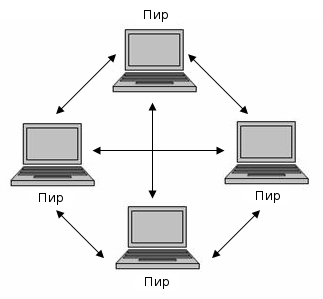
\includegraphics[width=0.6\linewidth]{peer}}
\caption{Организация peer-to-peer сети}
\label{0:peer}
\end{figure}

При работе в рамках парадигмы Peer-to-Peer (сокращенно P2P) компьютеры обмениваются ресурсами непосредственно друг с другом, без использования центрального сервера. Подход P2P обеспечивает решение проблем, возникших в результате экспоненциального роста интернет-сетей и веб-контента. Применение P2P позволило множеству польователей, которые раньше были простыми потребителями информации, поучаствовать в предоставлении контента. В момент своего появления, P2P было скорее модным словом, чем продуманной концепцией. В результате мощного продвижения с помощью средств массовой информации, технология P2P распространилась в академических и промышленных кругах.

Основные достоинства одноранговых вычислительных систем:
\begin{itemize}
\item упрощается поддержка масштабируемости при значительном росте количества узлов в вычислительной сети; 
\item повышается отказоустойчивость сети, т.к. сбой любого вычислительного узла не может привести к остановке функционирования сети целиком.
\end{itemize}

Тем не менее, существует ряд препятствий при построении P2P сетей:
\begin{itemize}
\item при работе с P2P приложениями, вычислительный узел берет на себя функции как клиента, так и сервера. Это приводит к увеличению требований к производительности каждого компьютера, включенного в такую сеть.
\item низкая степень защищенности машин, участвующих в P2P сети объясняется тем, что они предоставляют открытый доступ к своим ресурсам (таким как такты процессора, определенные папки на жестком диске и т.п.). Таким образом, при отсутствии средств защиты, компьютеры, включенные в P2P подвержены риску взлома или заражения со стороны недобросовестных участников. 
\item при построении P2P сети приходится преодолевать возможную гетерогенность аппаратного и программного обеспечения ее потенциальных участников. Этот вопрос может быть решен путем применения таких технологий как XML, Java и т.д.
\item Основная проблема P2P сетей~--- это поиск доступных ресурсов без использования централизованной системы управления. Каждому узлу приходится производить поиск среди сотен и тысяч ресурсов внутри сети, что является очень трудоемкой и ресурсоемкой задачей.
\end{itemize}

\subsubsection{Сервис-ориентированная архитектура}
В начале 2000-х годов мировое бизнес-сообщество занялось разработкой следующего поколения спецификаций, призванных решить проблемы ранних стандартов распределенных объектных технологий посредством веб-сервисов и сервис-ориентированной архитектуры (Service-Oriented Architecture~--- SOA).

\begin{figure}[h]
\center{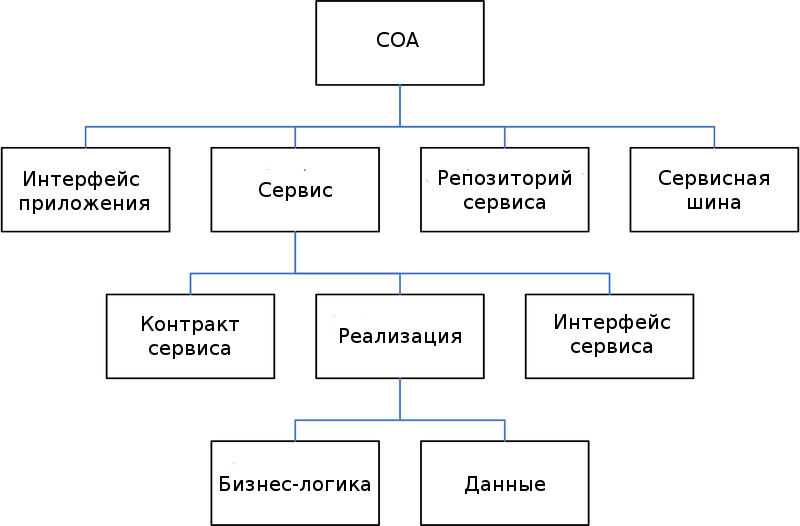
\includegraphics[width=1\linewidth]{soa}}
\caption{Одна из возможных реализаций архитектуры SOA}
\label{0:soa}
\end{figure}

Архитектура SOA не привязана к какой-либо определенной технологии. Она может быть реализована с использованием широкого спектра технологий, включая такие как REST, RPC, DCOM, CORBA или веб-сервисы. SOA может быть реализована, используя один из этих подоходов и, например, может использовать дополнительно механизм файловой системы для обмена данными.

Главное, что отличает SOA~--- это использование независимых сервисов с четко определенными интерфейсами, которые для выполнения своих задач могут быть вызваны неким стандартным способом, при условии, что сервисы заранее ничего не знают о приложении, которое их вызовет, а приложение не знает, каким образом сервисы выполняют свою задачу.

SOA также может рассматриваться как стиль архитектуры информационных систем, который позволяет создавать приложения, построенные путем комбинации слабо-связанных и взаимодействующих сервисов. Эти сервисы взаимодействуют на основе какого-либо строго определенного платформенно-независимого и языко-независимого интерфейса (например, WSDL). Определение интерфейса скрывает языко-зависимую реализацию сервиса.

Стандарты веб-сервисов были разработаны по инициативе организаций, занимающихся предоставлением удаленного доступа к определенным вычислительным ресурсам, и закреплены консорциумом W3C. К основным стандартам разработки и функционирования веб-сервисов можно отнести:
\begin{itemize}
\item SOAP~--- основанный на XML протокол взаимодействия веб-сервисов;
\item WSDL (Web Services Description Language~--- Язык описания веб-сервисов)~--- это методология описания ресурсов, предоставляемых веб-сервисом;
\item UDDI (Universal Description Discovery and Integration~--- Универсальный метод поиска и интеграции)~--- метод описания, поиска, взаимодействия и использования веб-сервисов. На сегодняшний день, сервис-ориентированный подход является стандартом «де-факто» при разработке распределенных вычислительных систем.
\end{itemize}

\subsubsection{Программные агенты}
Несмотря на все преимущества технологии веб-сервисов, они не предоставляют новых методологий и решений построения широкомасштабных вычислительных сетей. Для поиска решений в этом направлении, необходимо рассмотреть агентно-ориентированную парадигму построения распределенных вычислительных систем. Вычислительные сети на основе так называемых агентов~--- это принципиально иной подход к организации систем и приложений.

Технология прогрммных агентов является основой реализации данного дипломного проекта, и будет детально рассмотрена в следующей главе.
